%%%%%%%%%%%%%%%%%%%%%%%%%%%%%%%%%%%%%%%%%%%%%%%%%
%%         Projet Dome geodesique              %%
%%                                             %%
%%   Planète Sciences / InCOGnu / Tetalab      %%
%%%%%%%%%%%%%%%%%%%%%%%%%%%%%%%%%%%%%%%%%%%%%%%%%

%% Authors: Séverin Lemaignan


\documentclass[a4paper,12pt]{report}

\usepackage{fullpage}

\usepackage{graphicx}

\usepackage{xcolor}

\usepackage{ifthen}

\usepackage[utf8]{inputenc}

\usepackage[T1]{fontenc}
\pdfmapfile{+ubuntu-regular.map}
\pdfmapfile{+ubuntu-it.map}
\pdfmapfile{+ubuntu-bold.map}
\renewcommand{\rmdefault}{Ubuntu}

\usepackage{listings}
\usepackage{framed}
\usepackage{wrapfig}
\usepackage{fancyhdr} %headers and footers
\pagestyle{fancy}

\usepackage{url}
\usepackage{hyperref}
\usepackage{sectsty}

\usepackage{enumerate}

\usepackage{pdfpages} %% To add a cover to the doc
\usepackage{booktabs}
\usepackage{rotating}

% Fixme notes
\usepackage[draft,footnote,marginclue]{fixme}


\usepackage[french]{babel}

\graphicspath{{images/}}

%################# En-tête et pieds de page avec fancyhdr
\headheight=14.85pt
%pour récupérer les noms de section en minuscule
\renewcommand{\chaptermark}[1]{\markboth{#1}{}}
\renewcommand{\sectionmark}[1]{\markright{#1}}

\fancyhf{}
\fancyhead[RO,LE]{\bfseries\leftmark}
%\fancyhead[LE]{\rightmark}
\fancyfoot[LE,RO]{\bfseries\thepage}
\renewcommand{\headrulewidth}{0.3pt}
%\addtolength{\headheight}{2pt}
\addtolength{\headsep}{20pt}
\addtolength{\footskip}{10pt}
\renewcommand{\footrulewidth}{0pt}
\fancypagestyle{plain}{\fancyhead{}\renewcommand{\headrulewidth}{0pt}}

%%%%%%%%%%%%%%%%%%%%%%%%%%%%%%%%%%%%%%%%%%%%%%%%%%%%%%%%%%%%%%%%%%%%%%%%%%%%%%%%%
%%%%%%%%%%%%%%%%%%%%%%%%%%%%%%%%%%%%%%%%%%%%%%%%%%%%%%%%%%%%%%%%%%%%%%%%%%%%%%%%%

\title{
	
\includegraphics[width=12cm]{logos.pdf}\\
	\vfill
	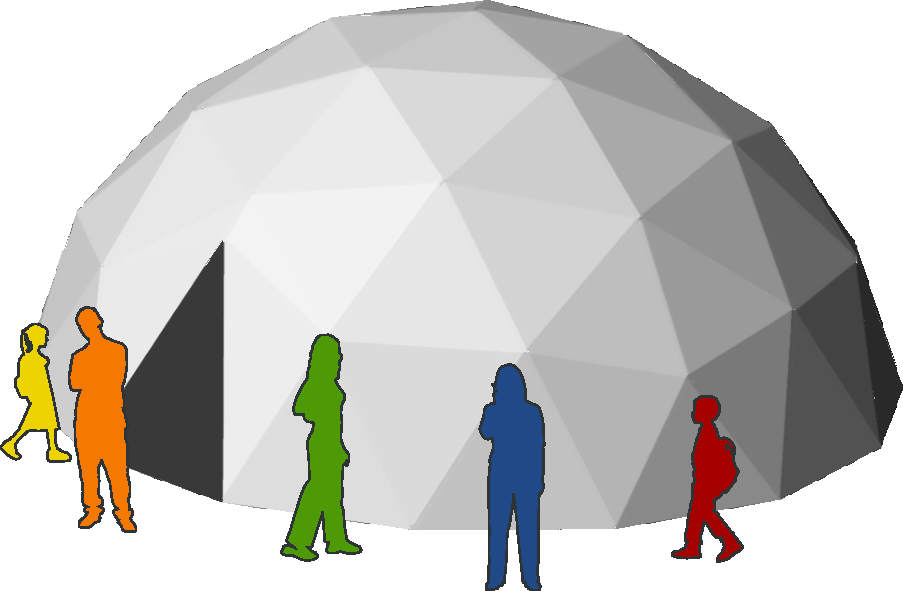
\includegraphics[width=9cm]{general.pdf}\\
	\vspace{3em}
	\LARGE{\textbf{Dôme géodésique}}\\[1cm]
	\large{Projet inter-associatif d'espace d'expérimentation et de projection}\\[1cm]
	\vfill
}

\author{
Séverin Lemaignan
}

%%%%%%%%%%%%%%%%%%%%%%%%%%%%%%%%%%%%%%%%%%%%%%%%%%%%%%%%%%%%%%%%%%%%%%%%%%%%%%%%%
%%%%%%%%%%%%%%%%%%%%%%%%%%%%%%%%%%%%%%%%%%%%%%%%%%%%%%%%%%%%%%%%%%%%%%%%%%%%%%%%%
\begin{document}

\IfFileExists{cover.pdf}{
\includepdf[pages=-, fitpaper]{cover.pdf}
\thispagestyle{empty}
\cleardoublepage
}

\maketitle

\tableofcontents

%%%%%%%%%%%%%%%%%%%%%%%%%%%%%%%%%%%%%%%%%%%%%%%%%%%%%%%%%%%%%%%%%%%%%%%%%%%%%%%%%
%%%%%%%%%%%%%%%%%%%%%%%%%%%%%%%%%%%%%%%%%%%%%%%%%%%%%%%%%%%%%%%%%%%%%%%%%%%%%%%%%

\chapter{Le projet Dôme}

\begin{figure}[!h]
\centering
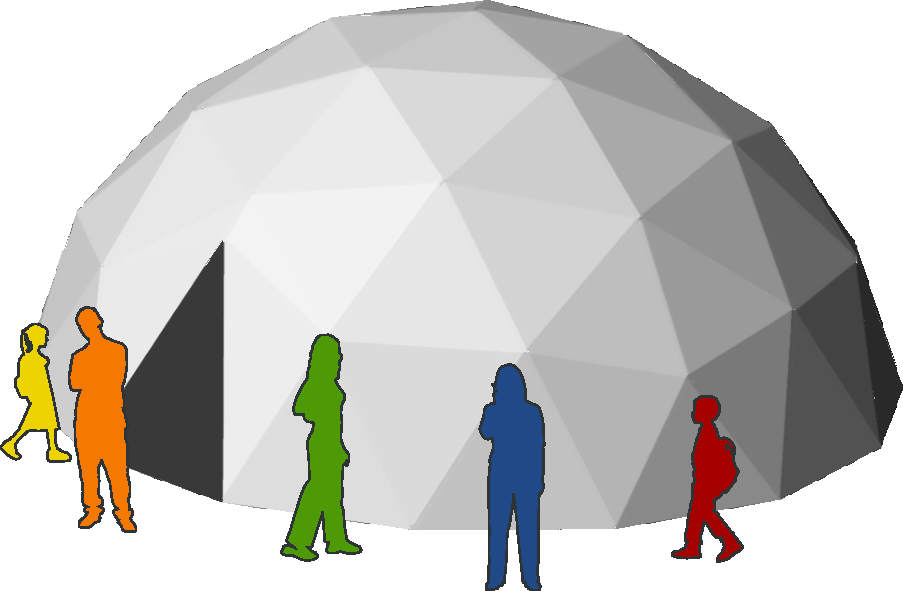
\includegraphics[width=9cm]{general.pdf}
\end{figure}


Lors d'une formation organisée à Planète Sciences courant 2011 est née l'idée,
entre bénévoles du Tétalab et de Planète Sciences, de construire un dôme
hémisphérique pour réaliser des projections vidéos immersives. Par ailleurs, au
même moment, des bénévoles de l'association InCOGnu réfléchissaient à se
procurer un dôme pour répliquer l'expérience du Cerveaurium...

Ce projet s'est ainsi construit avec les envies partagées de ces trois
associations.

Le dôme est une grande structure hémisphérique de 8m de diamètre, prévu pour
pouvoir être installé et démonté en quelques heures, et ainsi déplacé entre les
associations, en fonctions des manifestations, ateliers ou spectacles organisés
par chacunes.

Au moins trois types d'activités peuvent y être envisagées:

\begin{itemize}

	\item lors de manifestations associatives publiques, le dôme peut être une
	zone d'accueil du public, avec un caractère inhabituel et donc attirant. Il
	peut aussi être un espace remarquable pour des ateliers. De part sa forme
	et sa taille, il invite aussi à être utilisé comme point central lors de
	l'installation de manifestations avec de nombreux stands ou tentes.

	\item le dôme sera équipé d'une couverture opaque, bien adaptée à des
	projections vidéos immersives ``à 360''. C'est l'utilisation originale
	prévue pour le dôme. L'équipement de projection adéquat (lentille
	hémisphérique, vidéo-projecteur) fait parti du présent projet.  De nombreux
	types de projections sont possible, de films "standards" à des
	environnements 3D dynamiques et interactifs en passant par des applications
	type planétarium. La section suivant décrit quelques expériences possibles.

	\item enfin, le dôme est aussi envisagé comme une plateforme
	d'expérimentation inter-associative : c'est un espace atypique, modulable,
	créé par et pour les bénévoles des trois associations.  Nous aimerions
	qu'il devienne un endroit de création de contenus artistiques et
	scientifiques (en fonction des spécificités de chaque association) où
	puissent aussi avoir lieu des rencontres et des échanges de savoir-faire.
	Un espace expérimental ouvert.

\end{itemize}


\chapter{Description technique}

Le dôme mesure 8m de diamètre sur environ 3,2m de haut. Il permettera
d'accueillir confortablement 25 adultes debout.

\begin{figure}[!h]
\centering
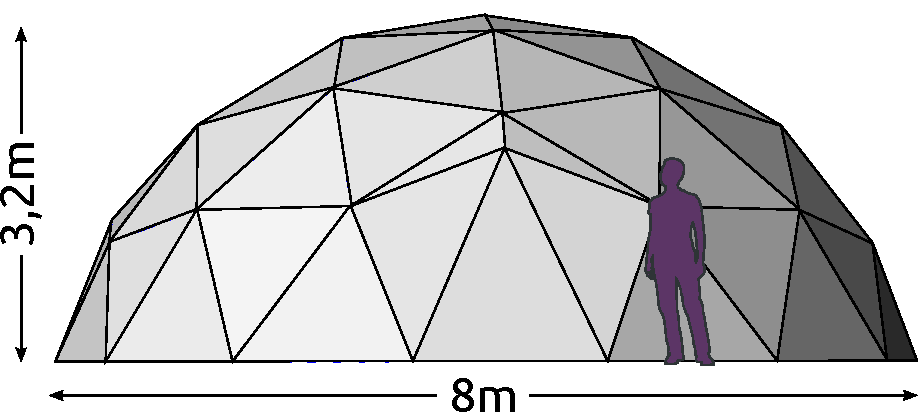
\includegraphics[width=9cm]{dimensions.pdf}
\end{figure}

Le dôme est composé d'une structure métallique tubulaire couvert d'une bâche
servant de support de projection.

\begin{figure}[!h]
\centering
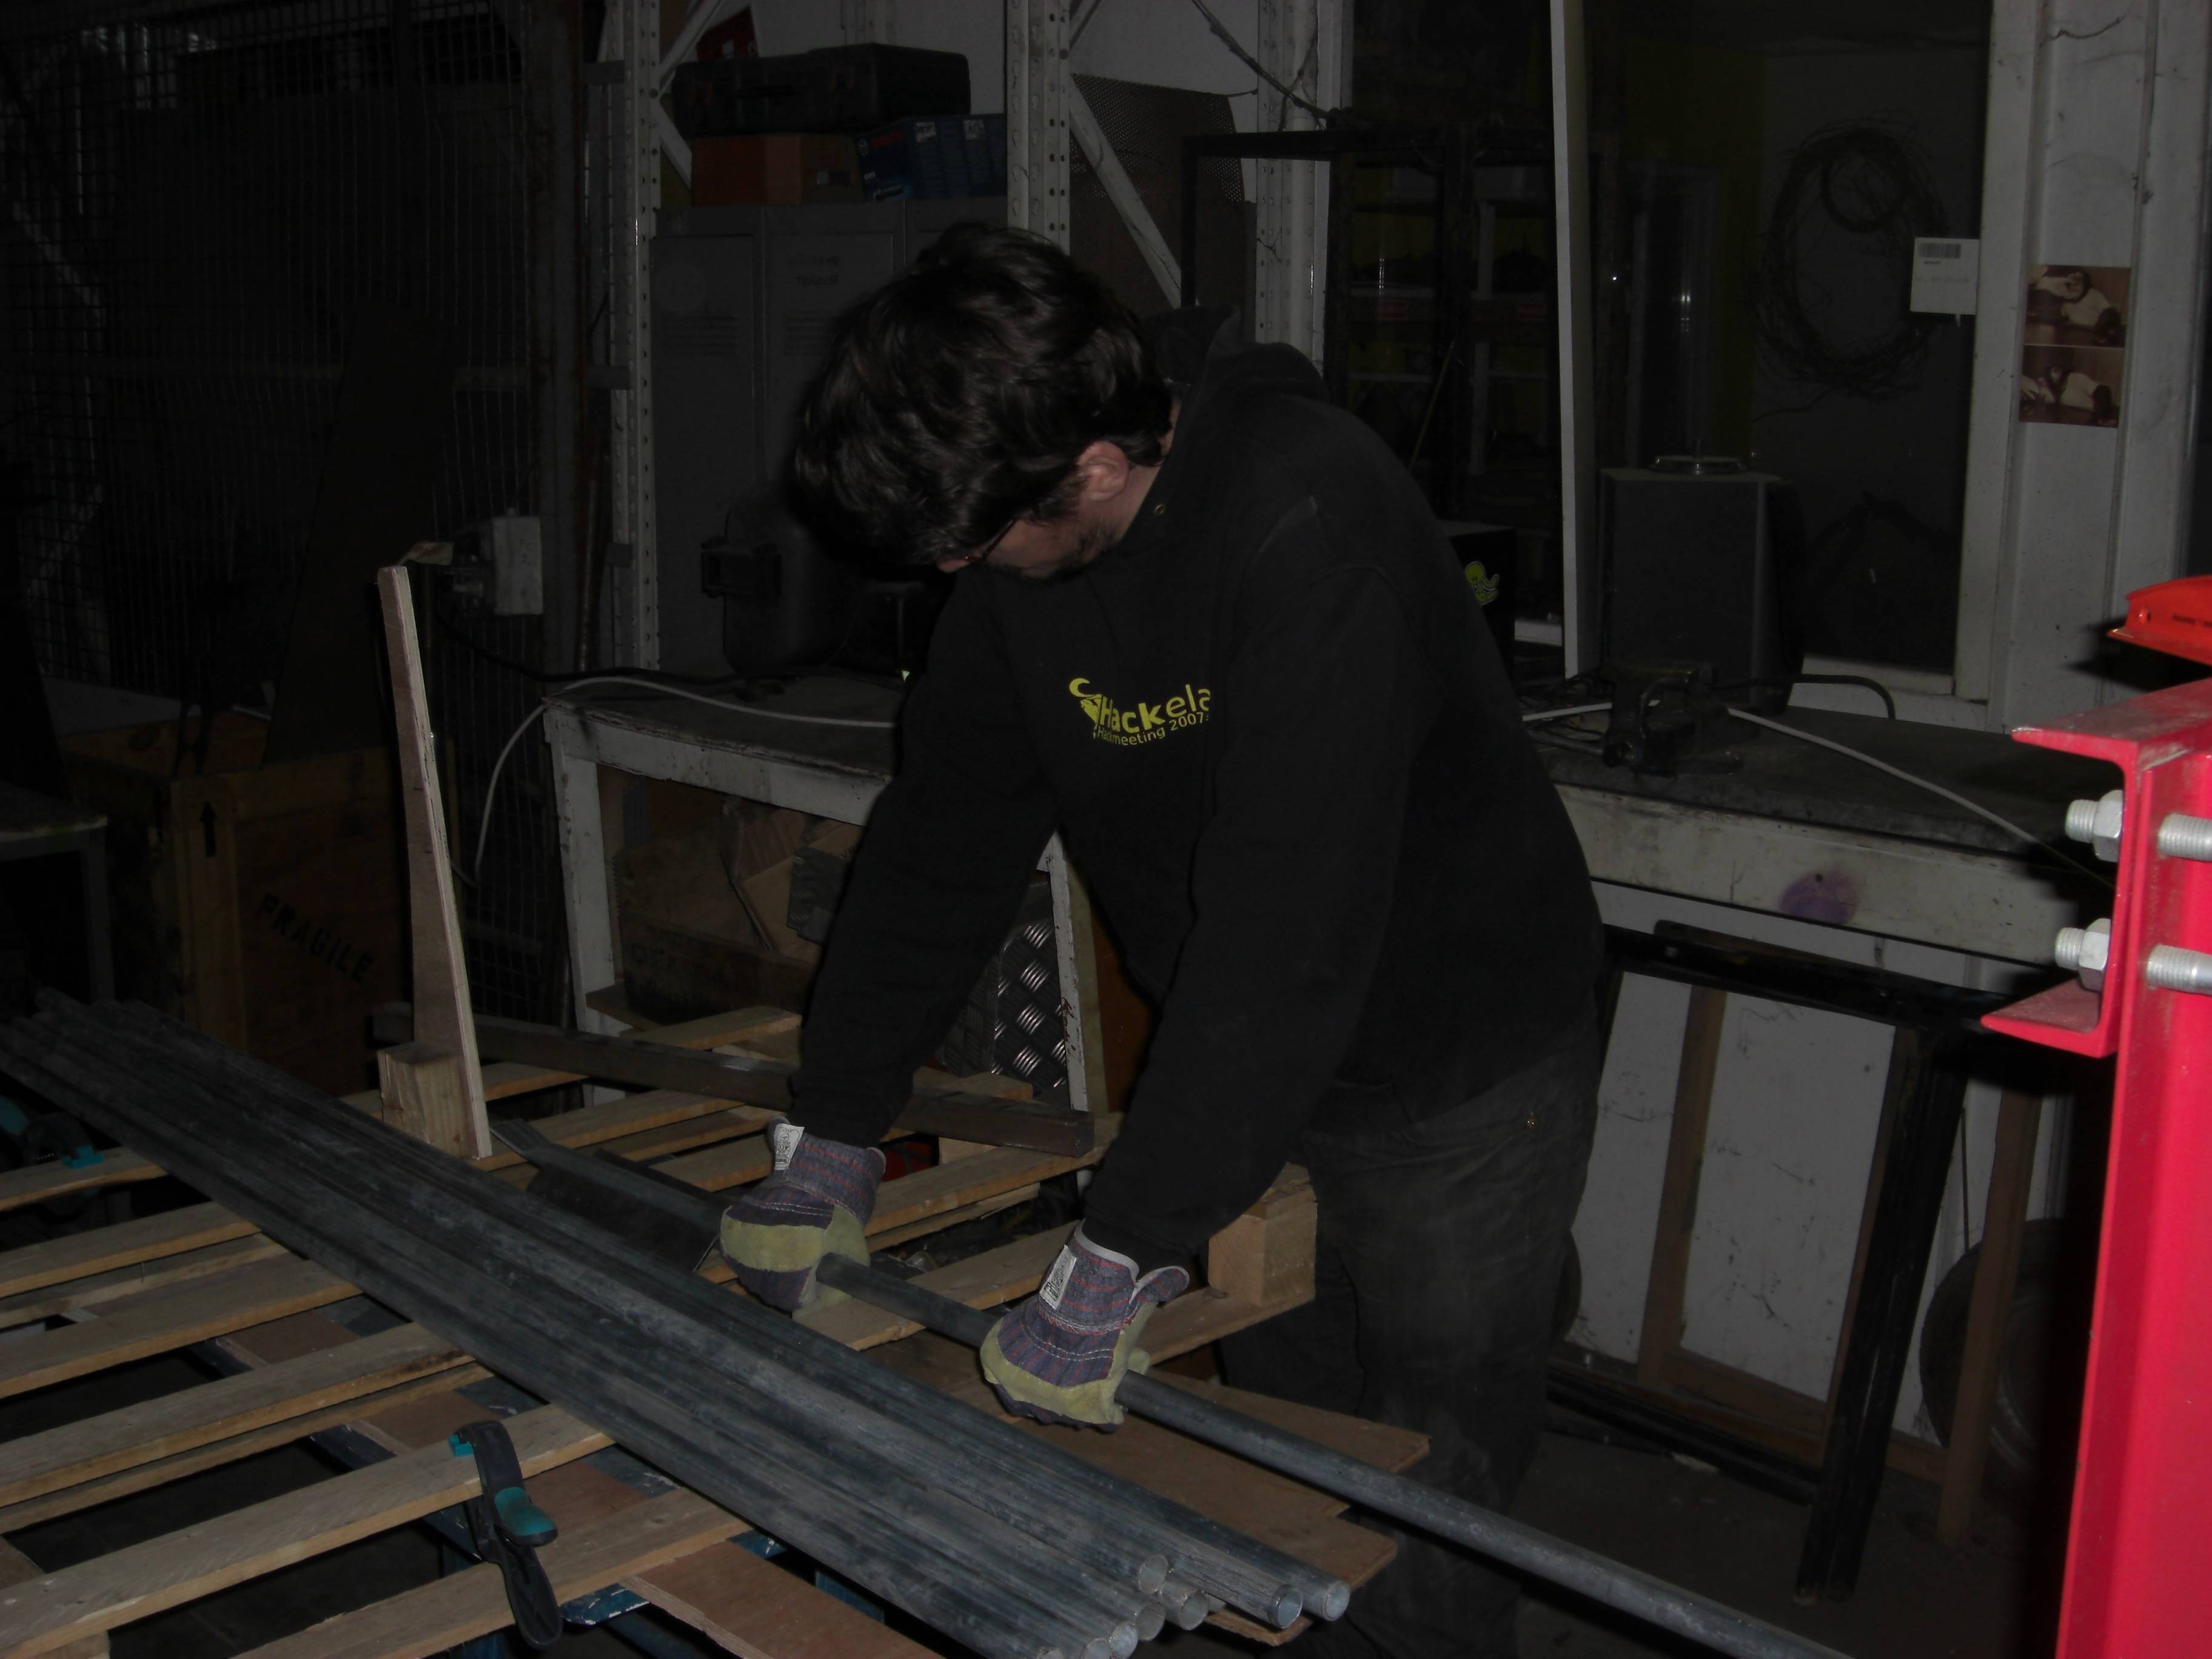
\includegraphics[width=9cm]{pliage_tubes.jpg}
\caption{Préparation des tubes : pressage des extrémitée, pliage, et perçage.}
\end{figure}

Le projet inclut aussi un certain nombre de composants dédiés à la projection hémisphérique.

\section{Structure}

La structure du dôme est composée de 120 tubes d'acier de 25mm de diamètre.  Il
y a principalement 3 longueurs (1,43m, 1,65m et 1,69m), plus 4 tubes de 2,25m
et 0,45m autour de la porte.

Ils sont assemblés en 45 points par des vis, formant au total 75 triangles
(figure~\ref{plan_assemblage}).

La structure étant en acier, elle est relativement lourde, mais résistante (un
adulte peut monter dessus sans problème).

\begin{figure}
	\centering 
	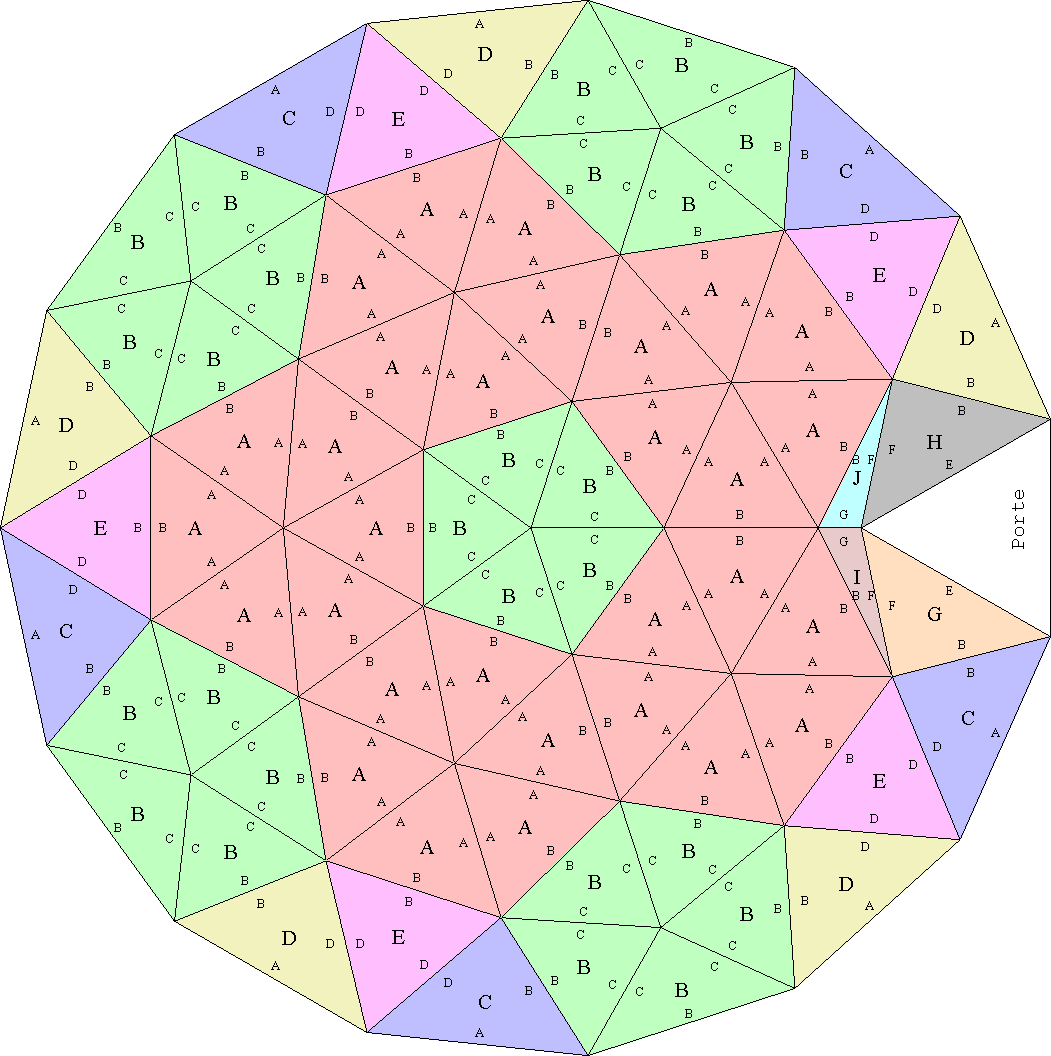
\includegraphics[width=9cm]{plan_assemblage.pdf}
	\caption{Plan d'assemblage du dôme. Les couleurs correspondent aux triangles
	identiques.} 
	\label{plan_assemblage} 
\end{figure}

\section{Surface de projection}

Le dôme est recouvert d'une bâche opaque, imperméable et blanche.  La bâche
assure le double de rôle de surface de projection et de parois occultante.

Par ailleurs, la bâche est choisie pour permettre l'accueil de public
(catégorie anti-feu M2).

\subsection*{Extensions}

Il est envisagé, à moyen terme, que des bâches ou secteurs de bâche puisse être
remplacé, en fonction des ambiances souhaitées, par des bâches
semi-transparentes et/ou colorées.

Il est de plus prévu que le dôme puisse être recouvert, selon les besoins, de décors
particuliers : l'association InCOGnu envisage par exemple la possibilité de
créer une coque en forme de cerveau (figure~\ref{coque_cerveau}).

\begin{figure}[!h]
\centering
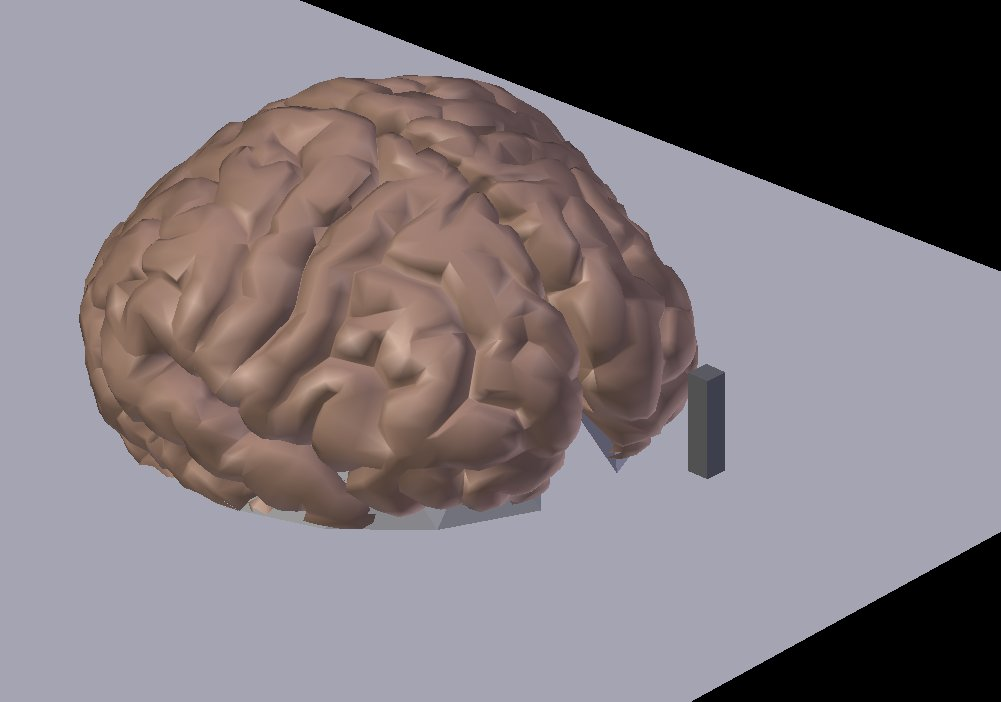
\includegraphics[width=9cm]{coque_cerveau.jpg}
\caption{Pré-projet de "coque cerveau" venant se placer sur le dôme}
\label{coque_cerveau}
\end{figure}

Ces extensions ne font pas partie du présent projet.

\section{Équipement}

Le dôme est équipé avec un système de projection hémisphérique basé sur un
vidéo-projecteur haute-définition dont l'image est diffusé à travers une
lentille {\it fish-eye}.

Le projecteur permet le branchement d'un ordinateur standard.

INSERT PHOTO MONTAGE FISH EYE

Le dôme dispose aussi de cinq spots contrôlés par un variateur, permettant de
piloter facilement l'ambiance lumineuse du dôme.

Par ailleurs, l'alimentation électrique des différents matériels utilisés à
l'intérieur du dôme est assurée par un boitier électrique central, équipé d'un
disjoncteur.

\chapter{Sécurité}

Le dôme est destiné à accueillir du public. Sa capacité maximale est estimée à
\textbf{25 adultes} simultanément.

C'est un ERP (Établissement Recevant du Public) de type \textbf{CTS}
(Chapiteaux, Tentes et Structures toiles), de 5ème catégorie (moins de 50
personnes).

En tant qu'ERP de 5ème catégorie, le dôme ne requiert pas, par lui-même, le
passage d'une commission de sécurité avant d'accueillir du public. Dans le cas
d'une utilisation du dôme au sein d'une manifestation plus large, la situation
peut être différente.

Référence: Article R123-1 du code de la construction et de l'habitation,
\url{http://www.legifrance.gouv.fr/WAspad/UnCode?&commun=CCONST&code=CCONSTRL.rcv}

\chapter{Activités prévues et envisagées}

\section{Activités scientiques}

Les associations Planète Sciences et InCOGnu ont comme raison première la
diffusion de la culture scientifique.

Parmis les utilisations du dôme envisagées par ces associations :

\begin{itemize}
	\item Planète Sciences a une importante activité en astronomie. Le dôme
	pourra servir de planétarium. Des logiciels libres comme Stellarium peuvent
	facilement être utilisés comme source vidéo à cette fin.

	\item L'atelier Cerveaurium : cette expérimence consiste à montrer, en
	direct, l'activité cérébrale de l'homme via un casque EEG (qui mesure
	l'activité électrique à la surface de la tête). Les signaux mesurés sont
	convertis en une carte d'activité du cerveau, projetée sur le dôme. Ce
	projet à été conçu et développé par Romain Grandchamp au sein de
	l'association InCOGnu.

    \begin{figure}[!h]
    \centering
    \includegraphics[width=4cm]{tete.jpg}
	\caption{Exemple de carte d'activité cérébrale calculée en temps réel et re-projetée.}
    \end{figure}


	\item Parmis les projets possibles à moyen terme, le dôme pourrait être
	utilisé dans un cadre mixte robotique/astronomie pour simuler une mission
	d'exploration planétaire : les enfants envoient et pilotent de l'extérieur
	un robot qui part en exploration à l'intérieur du dôme, préalablement
	aménagé pour simulé l'environnement d'une planète, imaginaire ou non.
	Charge aux enfants de déterminer si cette planète à de l'eau, de la vie,
	une atmosphère, etc.

\end{itemize}

\section{Activités artistiques}

\section{Autres activités}

De part son apparence particulière qui suscite la curiosité, le dôme peut être
un endroit particulièrement adapté à l'accueil de public lors de manifestations
généralistes où nos associations ont besoin de visibilité (type forum des
association). De même, lors de grosses manifestations, le dôme peut faire
office de "point accueil/information" facile à repérer.

Enfin, comme mentionné plus haut, le dôme se veut aussi un espace associatif
ouvert aux expérimentations. Il est donc prévu qu'il soit facilement disponible
pour les bénévoles de chacune des associations, hors des temps manifestations.
Nous espérons qu'il sera aussi l'occasion de favoriser les échanges et nouer
des partenariats forts entre nos associations.

\begin{figure}[!h]
\centering
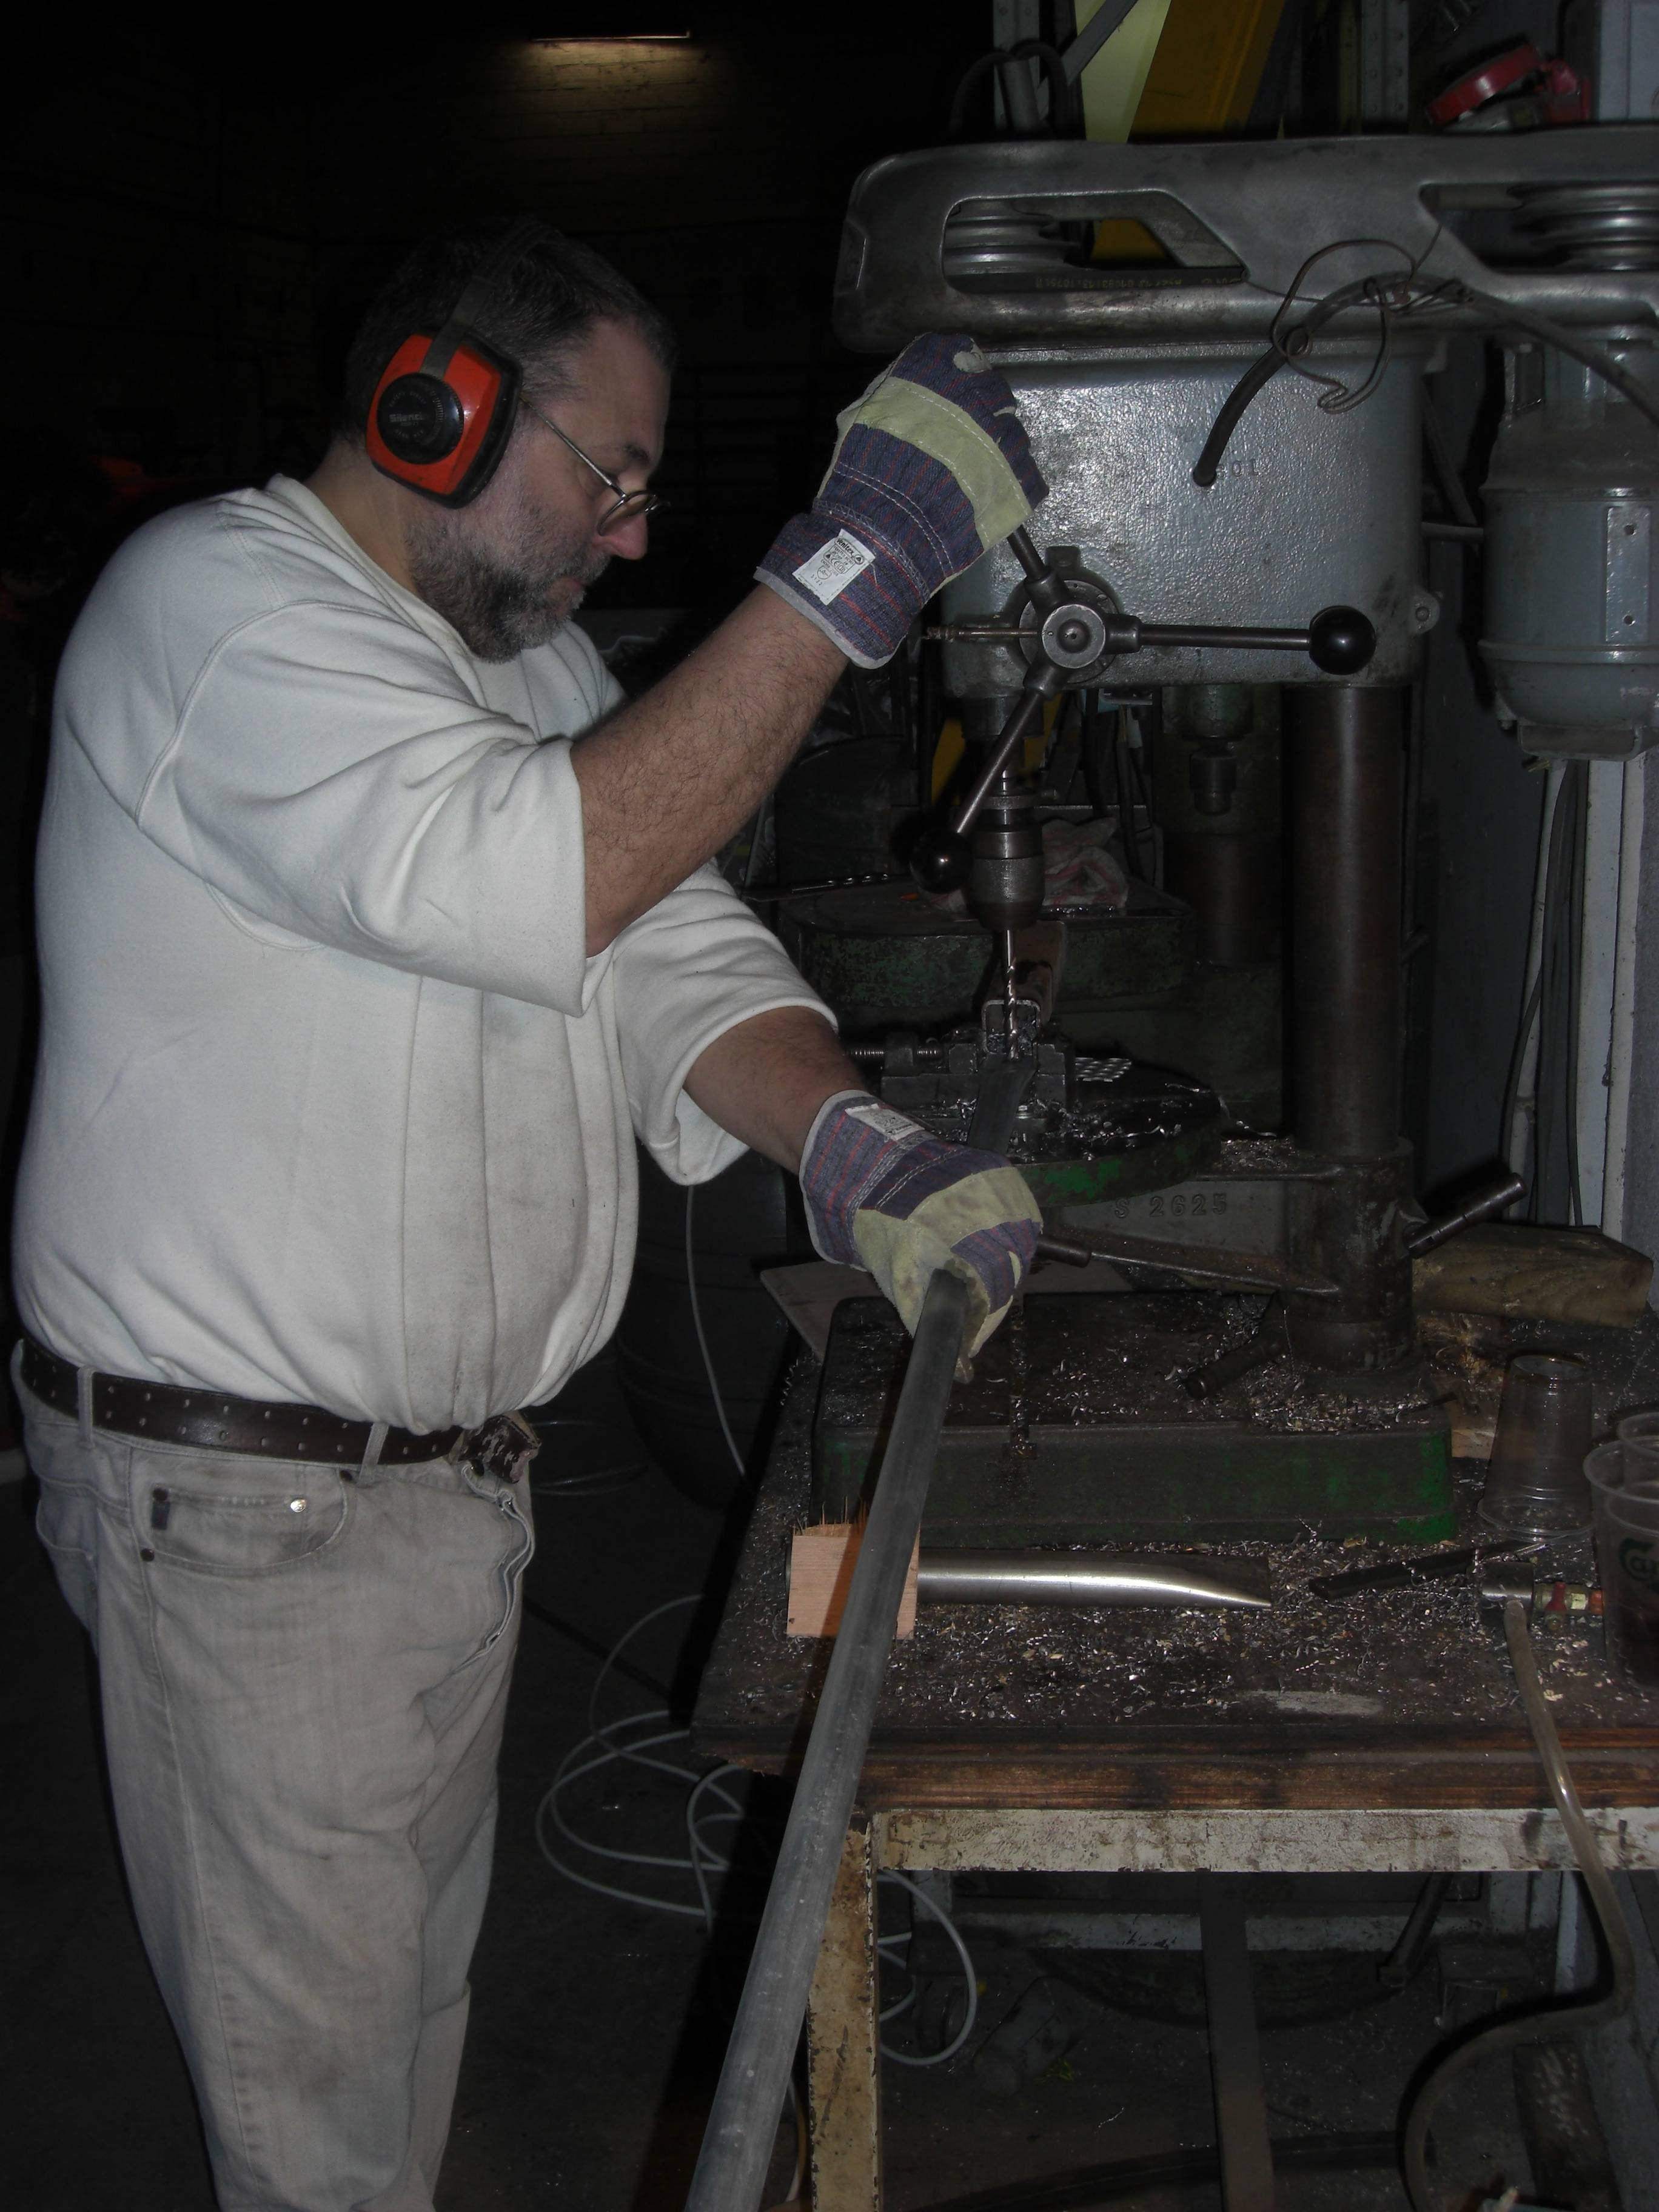
\includegraphics[width=9cm]{percage.jpg}
\end{figure}


\chapter{Budget prévisionnel}

%\begin{sidewaystable}
\begin{center}
\begin{tabular}{lrlr}
    \toprule
    Intitulé      & Montant \\
    \midrule
    
    \textbf{Dôme}                         &          \\
    \phantom{ZZ}Tubes acier               &    300   \\
    \phantom{ZZ}Peinture                  &     50   \\
    \phantom{ZZ}Visserie                  &     50   \\
    \phantom{ZZ}Bâche                     &   1500   \\
    \textit{Sous-total dôme}              & \underline{1900} \\
    
    \textbf{Équipement général}           &          \\
    \phantom{ZZ}Boitier électrique        &    300   \\
    \phantom{ZZ}Spots (5) + variateurs    &    200   \\
    \textit{Sous-total équipement}        & \underline{500} \\

    \textbf{Équipement projection}        &           \\
    \phantom{ZZ}Vidéoprojecteur           &    1500   \\
    \phantom{ZZ}Lentille fish-eye         &     150   \\
    \phantom{ZZ}Matériel optique          &     250   \\
    \textit{Sous-total vidéo}             & \underline{1900} \\
    
    \textbf{Outillage}                    &           \\
    \phantom{ZZ}Presse                    &     200   \\
    \phantom{ZZ}Petit outillage (pinceaux...) &  50   \\
    \textit{Sous-total outillage}         & \underline{250} \\
    
    \textbf{Total}                        & \fbox{4550} \\
    \bottomrule                
    \end{tabular}

\end{center}    
%\end{sidewaystable}

\chapter{Annexe : proposition de convention inter-associative}

\IfFileExists{convention.pdf}{
\includepdf[pages=-, frame=true]{convention.pdf}

}

%%%%%%%%%%%%%%%%%%%%%%%%%%%%%%%%%%%%%%%%%%%%%%%%%%%%%%%%%%%%%%%%%%%%%%%%%%%%%%%%%%%%%%%%%%%%%%%%%%%%%%%
\clearpage
\thispagestyle{empty}
~
\vfill
\begin{center}
	L'ensemble de ce projet est diffusé sous license libre Creative Commons Paternité-Partage à l'identique.\\
	\vspace{2cm}
	
\includegraphics[scale=0.5]{logo_cc.png}
\end{center}

\vfill

\begin{center}
	Les sources de ce document peuvent être téléchargées depuis le site GitHub.
	\url{http://github.com/skadge/dome/}
\end{center}

\vfill

\end{document}

